\documentclass{standalone}
\usepackage[libertine,varg]{newtxmath}
\usepackage{ebgaramond}
\usepackage{tikz}
\begin{document}
	\begin{tikzpicture}
		% coax
		\node at (0,6) {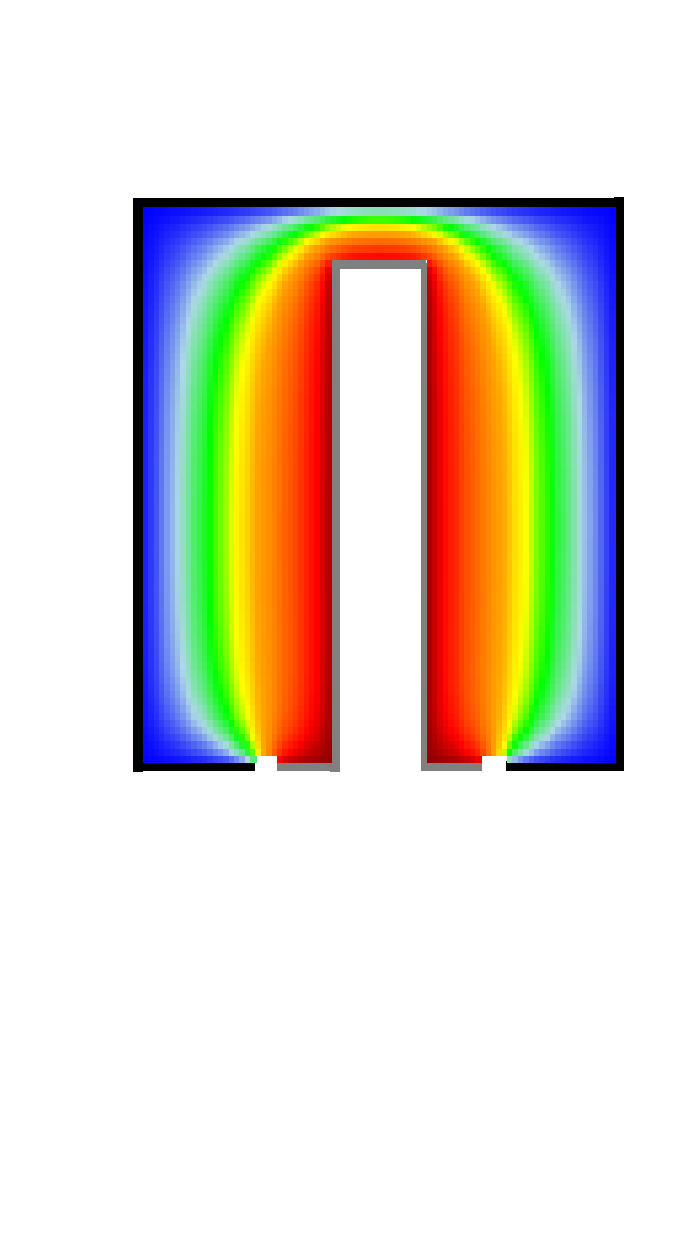
\includegraphics[width=5.9cm]{coax_base.pdf}};
		\node[rotate=90] at (-3.2,6) {coaxial};
		\node at (0,+9.6) {\color{black!30!green}n$^+$};
		\node at (0,6) {\color{red}p$^+$};

		% bege
		\node at (0,0) {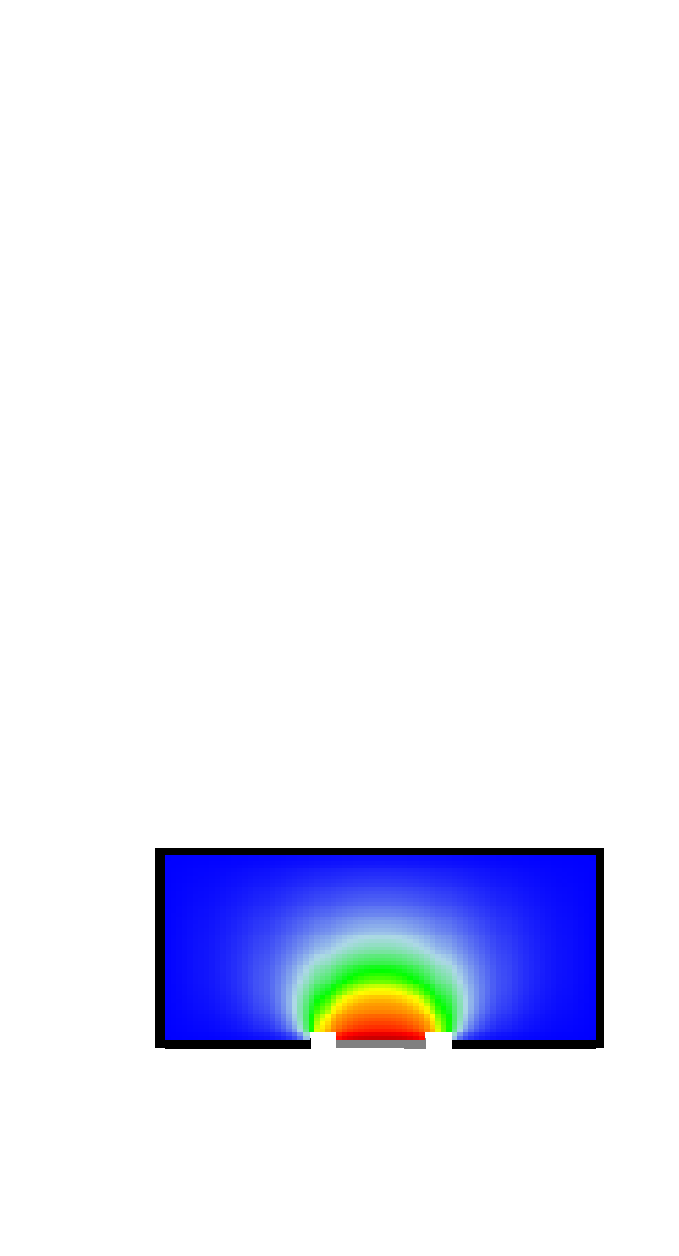
\includegraphics[width=6cm, angle=180]{bege_base.pdf}};
		\node[rotate=90] at (-3.2,0) {BEGe};
		\node at (0,+1.6) {\color{red}p$^+$};
		\node at (0,-1.5) {\color{black!30!green}n$^+$};
		% remove stupid line
		\node[fill=white] at (0.2,1.51) {\color{white}a};

		% arrows
		\node(a) at (-2.4,1.9) {groove};
		\node(b) at (-0.75,1.2) {};
		\node(c) at (-1.3,2.7) {};
		\draw[->] (a.east) to [out=0, in=90] (b.center);
		\draw[->] (a.east) to [out=0, in=270] (c.center);
		
		\node(d) at (2.4,1.9) {groove};
		\node(e) at (0.75,1.2) {};
		\node(f) at (1.4,2.7) {};
		\draw[->] (d.west) to [out=180, in=90] (e.center);
		\draw[->] (d.west) to [out=180, in=270] (f.center);
	\end{tikzpicture}
\end{document}
